% !TeX root = ../main.tex

\chapter{主要研究方法及技术路线}

\section{现有工具漏洞检测能力}

在开始进行实验之前,我们需要对现有工具的检测能力进行充分地调研。只有在了解现有工具的检测能力、检测特点的情况下,我们才能开始进行漏洞标准库的构建和新工具的研发工作。为此,我们调研了当下对\emph{Solidity}的研究工作,有的工作来自于商业团队,有的来自于学术团队;有的工具已经开源,并具备一定的社区影响力,有的工具发表于计算机顶级国际会议,带来了巨大的科研价值。发表于国际会议的工作,有的没有开源,对于这些没有开源的工作,虽然有论文做详细的说明,但由于不能获取到源代码,我们没办法对系统的内核做更深一步的分析,所以这些工具尽管有一定的学术影响力,我们也只能放弃。对于已经开源的工作,有些工具的开发逻辑不够严谨,或者相关文档不够完备,这些工具我们虽然能取得它们的源代码,但由于无法清晰地分析系统实现,故这些工具我们也无法很好地去分析他们的检测原理和检测能力。综上,在经过我们的筛选后,我们对如下工具在主要漏洞上的检测能力做出了总结,并和我们的系统\textsc{Athena}做比较列于表\ref{tab:detection_capability}。

\begin{table}
  \centering\small
  \caption{现有工具对于主要漏洞的检测能力总结}
  \begin{tabular}{cccccc}
    \toprule
    % after \\: \hline or \cline{col1-col2} \cline{col3-col4} ...
     & \textsc{Slither} & \textsc{Oyente} & \textsc{Smartcheck} & \textsc{Securify} & \textsc{Athena} \\
     \midrule
    可重入漏洞 & $\checkmark$ & $\checkmark$ & $\times$ & $\checkmark$ & $\checkmark$ \\
    意外异常漏洞 & $\checkmark$ & $\times$ & $\checkmark$ & $\times$ & $\checkmark$ \\
    低级调用漏洞 & $\checkmark$ & $\times$ & $\checkmark$ & $\times$ & $\checkmark$ \\
    自毁漏洞 & $\checkmark$ & $\times$ & $\times$ & $\times$ & $\checkmark$ \\
    \bottomrule
  \end{tabular}
  \label{tab:detection_capability}
\end{table}

上表所列的工具皆为静态分析工具,其中\textsc{Oyente}主要使用符号执行分析技术;\textsc{Securify}主要把代码转换成Datalog语言,并使用\textsc{Souffle}进行分析。\textsc{Slither}和\textsc{Smartcheck}采用的是传统的静态分析技术,即通过分析源代码得到程序的控制流图,并在控制流图上用预先设定好的匹配规则去寻找漏洞。从表中不难看出,使用传统静态分析技术的工具分析能力都比较不错,\textsc{Slither}支持我们提及的所有漏洞的检测,\textsc{Smartcheck}不支持两个漏洞的检测;而使用符号执行分析技术,包括使用其他静态分析技术的工具,对主要漏洞的支持都不太好,甚至只支持一个漏洞的检测。值得一提的是,这两个工具\textsc{Oyente}和\textsc{Securify}皆是在源代码编译之后产生的字节码上进行软件分析的,字节码的分析提供的信息更少,相比之下\textsc{Slither}和\textsc{Smartcheck}都是对源代码或者中间语言进行分析,故我们推测是由于技术路线的差异造成它们在不同漏洞上的分析难度不同,也就没办法支持所有漏洞的分析任务。

\section{使用克隆分析技术寻找漏洞代码}

在克隆代码分析技术中,按照代码相似的不同程度,我们可以把代码划分为以下几种克隆层次:
\begin{itemize}
  \item \textbf{第一类克隆:完全克隆。}这种克隆下层次下的相似代码之间完全相似,没有任何差异。
  \item \textbf{第二类克隆:重命名克隆。}这种克隆层次下的代码之间绝大部分相似,在类型、标识符、注释、空格之间有些许差异。
  \item \textbf{第三类克隆:重构克隆。}这种克隆层次下的相似代码之间具有结构层次的不同,例如缺少部分语句,多出部分语句,语句顺序不同等等。
  \item \textbf{第四类克隆:语义克隆。}这种克隆层次下的相似代码之间可能完全不同,但他们具有相同的语义,实现了相同的功能或流程。
\end{itemize}
从克隆层次的分类我们可以看出,第一类克隆和第二类克隆不涉及代码结构上的变化,因而能用比较简单的技术进行分析。在Kamiya等人的工作中\cite{ccfinder},使用了基于标记的克隆分析技术来寻找克隆代码,将代码的关键部分转换为标记,再在标记上进行分析寻找。由于前两类克隆代码的分析并没有什么挑战,因此现在已经有很多这方面的工作。对于第三类克隆,因为代码之间出现了语句结构的差异,例如多的语句,少的语句等等,直接借助基于标记的克隆分析技术来寻找克隆代码可能会遇上很多困难。为了解决这一问题,有人提出了提取代码特征转换成特征向量,并在高维空间进行比较的办法\cite{deckard},也有的工作提出使用软件的控制流图进行语句结构的比较\textcolor{red}{Add citation here}。而对于第四类克隆的分析,仍然是当前软件工程学界的一个有挑战的课题。有的工作提出使用深度学习算法进行代码语义的提取\textcolor{red}{Add ICST citation},但仍有很大的局限性如学习算法的数据集匮乏,很难找到数量充足且质量上乘的训练材料。因此,在讨论克隆分析技术时,我们主要解决的是寻找前三类克隆的相似代码的问题。

针对以上三种代码克隆等级,之前的工作提出了很多不同粒度的解决方案:
\begin{enumerate}
  \item \textbf{基于标记粒度的克隆分析技术:}使用基于标记力度的克隆分析技术试图使用将代码语句转换成标记序列,然后再在标记序列上比较相似度。这其中最出名的工作有CP-Miner\cite{cpminer}。CP-Miner解析了程序代码,并使用了“最频繁子序列挖掘”算法对代码生成的标记序列进行比较。这个算法由CloSpan\cite{clospan}这篇工作提出。多亏了CloSpan这篇工作在改进算法运行效率方面的贡献,CP-Miner可以在大规模代码,如Linux内核代码下仍保持了较低的内存占用。但是,CP-Miner的运行时间复杂度在最坏情况下为$\mathcal{O}(n^{2})$,$n$为代码行数,运行耗时较长。除开在大规模代码下的效率问题,CP-Miner也容易产生很多误报,这个是由于他们激进的代码抽象策略及有筛选的遗产算法导致的。虽然CP-Miner的开发者认为CP-Miner在数据集上的表现不错,但很明显CP-Miner并没有在漏洞代码检测这项任务上有足够的可靠行。
  \item \textbf{基于代码行粒度的克隆分析技术:}在ReDeBug\cite{redebug}中,分析系统将代码行的集合作为处理单元。系统驱使一个$n$行($n$默认为4)的窗口在源代码中滑动,并在每个窗口上使用三种不同哈希函数。该系统通过对比两文件各窗口的哈希值来计算文件之间的相似程度。虽然ReDeBug的这个特性使它能够检查一些第三类克隆的克隆代码,但它却无法检查那些第二类克隆,即变量名或者数据类型有变化的克隆代码。因此,ReDeBug会漏掉很多有漏洞但差异很小的克隆代码。更进一步,使用基于代码行粒度的克隆分析技术会导致上下文信息被局限一个很小的范围内,并最终导致引入了很多的误报。同时,ReDeBug需要花费大量的时间去处理源代码文件并建立哈希库,性能表现欠佳。
  \item \textbf{基于函数粒度的克隆分析技术:}SourcererCC\cite{sourcerercc}使用了基于函数粒度的克隆分析技术,试图来检测第三类克隆的克隆代码。它使用了标记集的检测技术解析了所有的函数,并针对每个函数的标记集建立了检索目录;然后,它寻找两个函数间相同的标记,并使用了\emph{Overlap}函数计算这两个函数之间的相似度。如果这个相似度超过了人为预先确定的一个阈值,则判断在这两个函数之间存在代码克隆现象。该系统在实现时,为了减少相似度的计算次数,对标记按出现的频数进行权重计算,出现频数高的标记获得较高权重,对持有较高权重的标记进行计算。但是,在权衡检测第三类克隆代码的能力与检查漏洞的能力时,SourcererCC对与漏洞代码的检测能力受到了很大的限制。在很多情况下,打过补丁的代码(安全代码)与未打补丁的代码(漏洞代码)之间的差距非常小,甚至只有一个\codeff{if}语句的差距,SourcererCC也无法检测这些漏洞代码。

      Yamaguchi等人提出使用漏洞推导的方法\cite{vul-extrapolation}来分析第四类克隆,即语义克隆的代码。他们分析函数的抽象语法树,并提取语法树的特征并将其嵌入向量空间中;在完成提取工作后,他们对高维向量使用奇异值分解来获取函数的结构信息。虽然他们的方法具备了检测一定程度的第四类克隆的能力,但是他们的系统运行流程有太多的时间和空间消耗,并且在论文中他们也没有明确给出这种技术的准确程度。

      我们必须指出,在使用高级别的代码抽象技术(标记序列,语法树)来分析克隆代码可能对分析代码克隆是有帮助的,但他们不足以准确地分析相似的漏洞代码,因为这些漏洞的语境通常会非常复杂。
  \item \textbf{基于文件粒度的克隆分析技术:}DECKARD\cite{deckard}对每个源代码文件都分别构建了抽象语法树,并从文件的抽象语法树上提取了特征向量,再在特征向量上使用欧几里得距离来进行聚类,经过聚类,欧氏距离较近的文件则被判断为克隆代码文件。这种基于语法树的方法需要大量的执行时间,因为子图同构是一个著名的NP完全问题。更进一步说,DECKARD并没有保证足够的扩展性,在面对大数据集时表现差强人意,同时,DECKARD也带来了很高的误报率,这也说明具有相同语法树结构的代码片段可能不是克隆代码。

      FCFinder\cite{fcfinder}去除了代码的注释、重复空格、换行,再对代码用MD5算法计算哈希值。它建立了一个哈希表,表的键值为文件名,数值为对应文件的哈希值。如果发现有文件的哈希值重复,则判断这几个文件为克隆代码文件。相比于DECKARD,FCFinder具有了良好的可扩展性。再FreeBSD软件上的克隆检测上,耗时更少,同时保持了一定的准确率。 可是,和DECKARD一样,它也不能很好地检测高度相似但具有微笑不同的克隆代码。
  \item \textbf{混合粒度的克隆分析技术:}有一些工作使用了几种不同粒度的克隆分析技术。VulPecker\cite{vulpecker}是一个能自动检查漏洞的软件分析系统。它给漏洞加上了事先定义好的特征,再根据代码的实际情况算则合适的代码相似度算法(如最长公共字串算法)计算代码相似度。在这个分析技术的帮助下,它找到了40个未被NVD(National Vulnerability Database)记录在案的漏洞。可是,这个系统在大量代码的情况下耗时过长,无法应对大量代码的检测任务。
\end{enumerate}

综上所述,对于不同粒度不同情况下的克隆代码分析,之前的工作做出了相当的努力。同时,我们也不难看出,要达成使用克隆分析技术来寻找代码漏洞的目标,我们不仅要保证我们的检测器具备一定的扩展性,以应对检测大量的代码的情况;其次我们也应该选用合理的代码抽象代码,来提取不同漏洞的特征,借助提取的特征来匹配相似的代码片段;最后,代码相似度计算算法的选择对分析克隆代码的能力至关重要,我们应该合理地选择代码相似度的计算算法。

\section{在智能合约软件上使用克隆分析技术的可行性}

在上一个部分我们调研了现有的软件克隆分析技术在不同的软件克隆等级上的效果和优缺点,我们也提出了要实现使用克隆分析技术去寻找漏洞代码,不仅要谨慎选择相似度算法,也必须保证系统即使在面对大量代码时也能维持较快的检测速度。但是,目前还没有工作在智能合约上使用克隆分析技术去寻找漏洞代码,因此,在这一部分,我们将证明在智能合约软件上使用克隆分析技术是可行的。

\subsection{智能合约代码相似度观察}
在我们观察了大量的智能合约软件代码过后,我们发现,在以太坊平台上存在着大量的代码克隆现象。在我们从Etherscan\footnote{一个提供智能合约数据及分析服务的网站。}上爬取了接近十万的智能合约代码,在使用最长公共字串来计算代码间相似度之后我们发现,统计代码相似度层级如下图\ref{fig:similarity}所示。
\begin{figure}[htbp]
\vspace{+2mm}
  \centering
  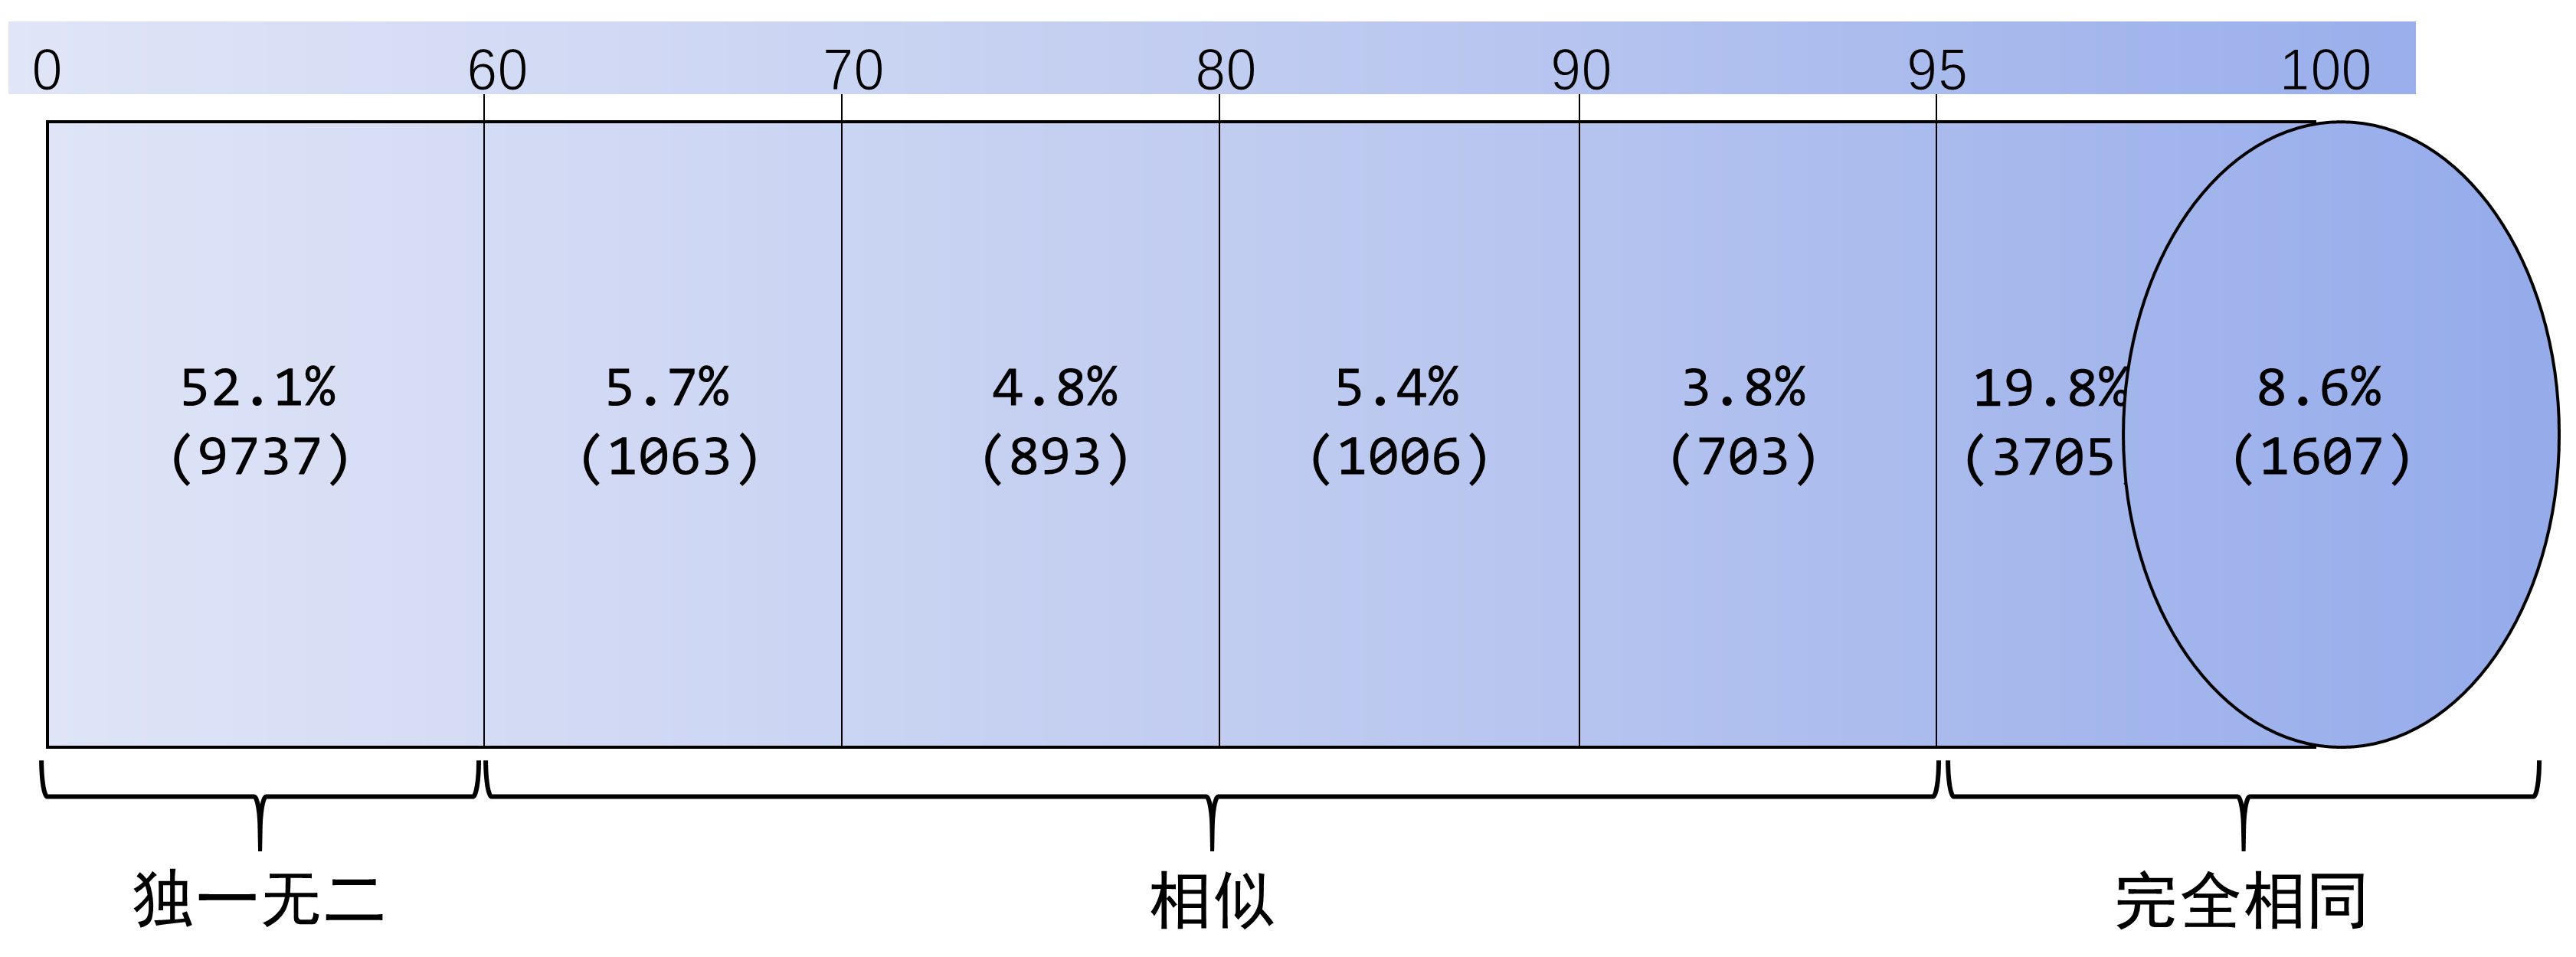
\includegraphics[width=0.9\textwidth]{figures/similarity.png}
  \caption{智能合约代码相似度统计}
  \label{fig:similarity}
\vspace{-5mm}
\end{figure}
我们可以明显看出,大部分智能合约软件内部存在着代码克隆现象,我们推测这是由于\emph{Solidity}代码无法引用代码引起的。很多智能合约软件直接复制已经存在的软件代码,稍加改动,如修改了交易地址,甚至不改动就添加到自己的代码中,参与自己软件的运行过程,如图\ref{fig:similar_code}所示。很明显,这虽然方便了开发者,减轻了开发任务,但是直接拷贝代码的行为容易在无意间引入漏洞。在一个存在很多克隆代码的平台,要保证软件的平均安全等级是很困难的。\emph{Solidity}研究团队推荐开发者拷贝或使用经过官方团队审计的接口代码,但是不推荐开发者拷贝其他任何代码。
\begin{figure}[H]
    \centering
    \begin{subfigure}{\linewidth}
    \centering
    \begin{minipage}{1.0\linewidth}
    \begin{lstlisting}
    contract BanyanIncomeLockPosition is Ownable {
    uint64 public unlockBlock = 8372051;
    address public tokenAddress = 0x35a69642857083BA2F30bfaB735dacC7F0bac969;
    ...
    }
    \end{lstlisting}
    %\caption{test}
    \end{minipage}
    \end{subfigure}
    \quad
    \begin{subfigure}{\linewidth}
    \centering
    \begin{minipage}{1.0\linewidth}
    \begin{lstlisting}
    contract BanyanIncomeLockPosition is Ownable {
    uint64 public unlockBlock = **6269625**;
    address public tokenAddress = **0x0a3f9678d6b631386c2dd3de8809b48b0d1bbd56**;
    ...
    }
    \end{lstlisting}
    %\caption{test}
    \end{minipage}
    \end{subfigure}
    \caption{相似代码示例,两个地址不同的智能合约软件仅有微小不同,不同之处已用**标出}
    \label{fig:similar_code}
\end{figure}

\subsection{智能合约克隆分析技术探究}
针对以太坊平台如此严重的代码克隆现象,我们提出使用代码克隆分析技术来寻找漏洞的方法。在VUDDY\cite{vuddy}这篇工作中,研发团队使用了根据漏洞代码的语法特征提取了漏洞的抽象表示,再通过相似度计算算法来寻找漏洞代码。VUDDY的这种技术,是从漏洞本身出发,寻找与漏洞相似代码的一种技术。这种方法具备良好的可扩展性,在寻找大量相似代码时也能保证令人满意的速度,在VUDDY的论文中,开发团队使用VUDDY完成了数以亿计行的代码的漏洞检测工作,并成功申请了数十个CVE\footnote{Common Vulnerabilities and Exposures,著名软件漏洞库和漏洞审计平台}。VUDDY的工作给了我们启发,在智能合约上,我们需要使用一种足够巧妙的方法去提取漏洞的抽象表现形式,抽象程度不能太高或者太低,太高会误报很多漏洞代码,太低则会漏掉很多真实的漏洞代码;我们还需要使用足够巧妙的代码相似度算法去计算代码之间的相似度,这种相似度计算方法必须和代码的抽象表现形式结合,不能有太高的时间复杂度;最后,我们需要对系统报告的漏洞做一定程度的人工分析,虽然在严谨的实验中,人工的行为容易带来实验结果的偏差,但是我们参与实验的检查人员都是智能合约、区块链及软件工程方面的领域专家,可以尽可能减少人工介入带来的偏差。那些经过人工检查,或者被系统报告有漏洞的代码,我们会用来不断地改进我们系统的检测能力,并建立漏洞标准库。

\subsection{结合克隆分析技术与字节码分析技术}
我们的系统不仅提供对智能合约源代码的漏洞检测功能,也能完成对字节码的反汇编任务以及控制流图分析。\textsc{Oyente}\cite{oyente}在字节码的基础上,使用了反汇编技术结合控制流图分析,并加上了符号执行分析技术,实现了漏洞的检测。无独有偶,之后的符号执行技术如\textsc{SCompile}\cite{scompile},\textsc{Manticore}\cite{manticore}也是在字节码上使用了符号分析技术,并结合自己确定的漏洞规则来进行检测。在我们的系统中,我们并不打算在字节码上加入符号分析技术并对字节码进行漏洞检测,我们只提供对字节码的代码结构静态分析,这是因为经过我们的广泛调研,如今字节码的反编译技术及语义解析技术并不是很成熟,我们觉得不足以支撑实现一个具有一定准确率的漏洞检测系统;其次,加入符号分析技术的工作量过大,超出了我们这篇论文的研究范畴,我们也希望相关同僚在字节码的漏洞分析检测技术上取得进一步的突破。

\subsection{漏洞检测系统结构设计}
我们给出了我们整体的系统结构,如图\ref{fig:system_diagram}所示。系统使用智能合约软件作为输入,分析结果及标准数据库作为输出。在系统的开始,会对输入的智能合约软件做相关检测,如果输入的智能合约软件为源代码形式,则进行源代码分析及进一步的漏洞检测;如果输入的智能合约软件为字节码形式,则对字节码进行反汇编,并将得到的汇编码作为输入进行控制流图分析,最后输出简单的分析结果。在源代码结束控制流图分析之后,我们将对软件进行漏洞规则匹配。漏洞靠目测给i哦则是经过我们智能合约领域专家总结得出的一套漏洞模板,并进行一定程度的抽象。再之后,我们用相似度算法计算漏洞规则与输入的控制流图进行相似度计算,如果得到的相似度高于我们设定好的阈值,我们就判断这是一个可疑的漏洞代码,我们将把这段代码保存并交由我们领域专家进行进一步检查。加入人工检查的目的是为了漏洞检测系统的公平公正,当下的对于智能合约漏洞检测的论文中对于漏洞的定义并不一致,且尚没有一个高度完备的工作能囊括所有的漏洞形式,因此,为了方便标准库构建和系统的优化,我们需要专家进行一定程度的人工干预,对系统的检测结果进行二次检测。如果专家检查到了系统的误报,说明我们总结的漏洞检测规则仍有不完备的地方,我们将根据误报的漏洞形式进一步完善系统的漏洞检测规则。漏洞检测规则的完善我们将根据漏洞的误报形式来决定,并不是所有的误报我们都要进行改进。这也是进行人工干预的优点,可以选择需要改进的地方进行恰当的改进。最后,对于那些系统正确判断的软件漏洞,我们将把漏洞代码加入漏洞库。漏洞库是我们标准库构建工作的结晶,经过不断修缮也能给后续的智能合约软件分析工作带来长远的便利。出于人道主义和安全考虑,我们并不会公开我们漏洞库的所有漏洞,但是我们会匿名掉关键信息并展示部分漏洞代码作为案例分析的一部分。随着和漏洞代码的作者联系不断进行,如果软件作者已经做出相关回应,修复了漏洞,我们也会在将来公开更多的漏洞代码用作学习和警示。
\begin{figure}[b]
\vspace{+2mm}
  \centering
  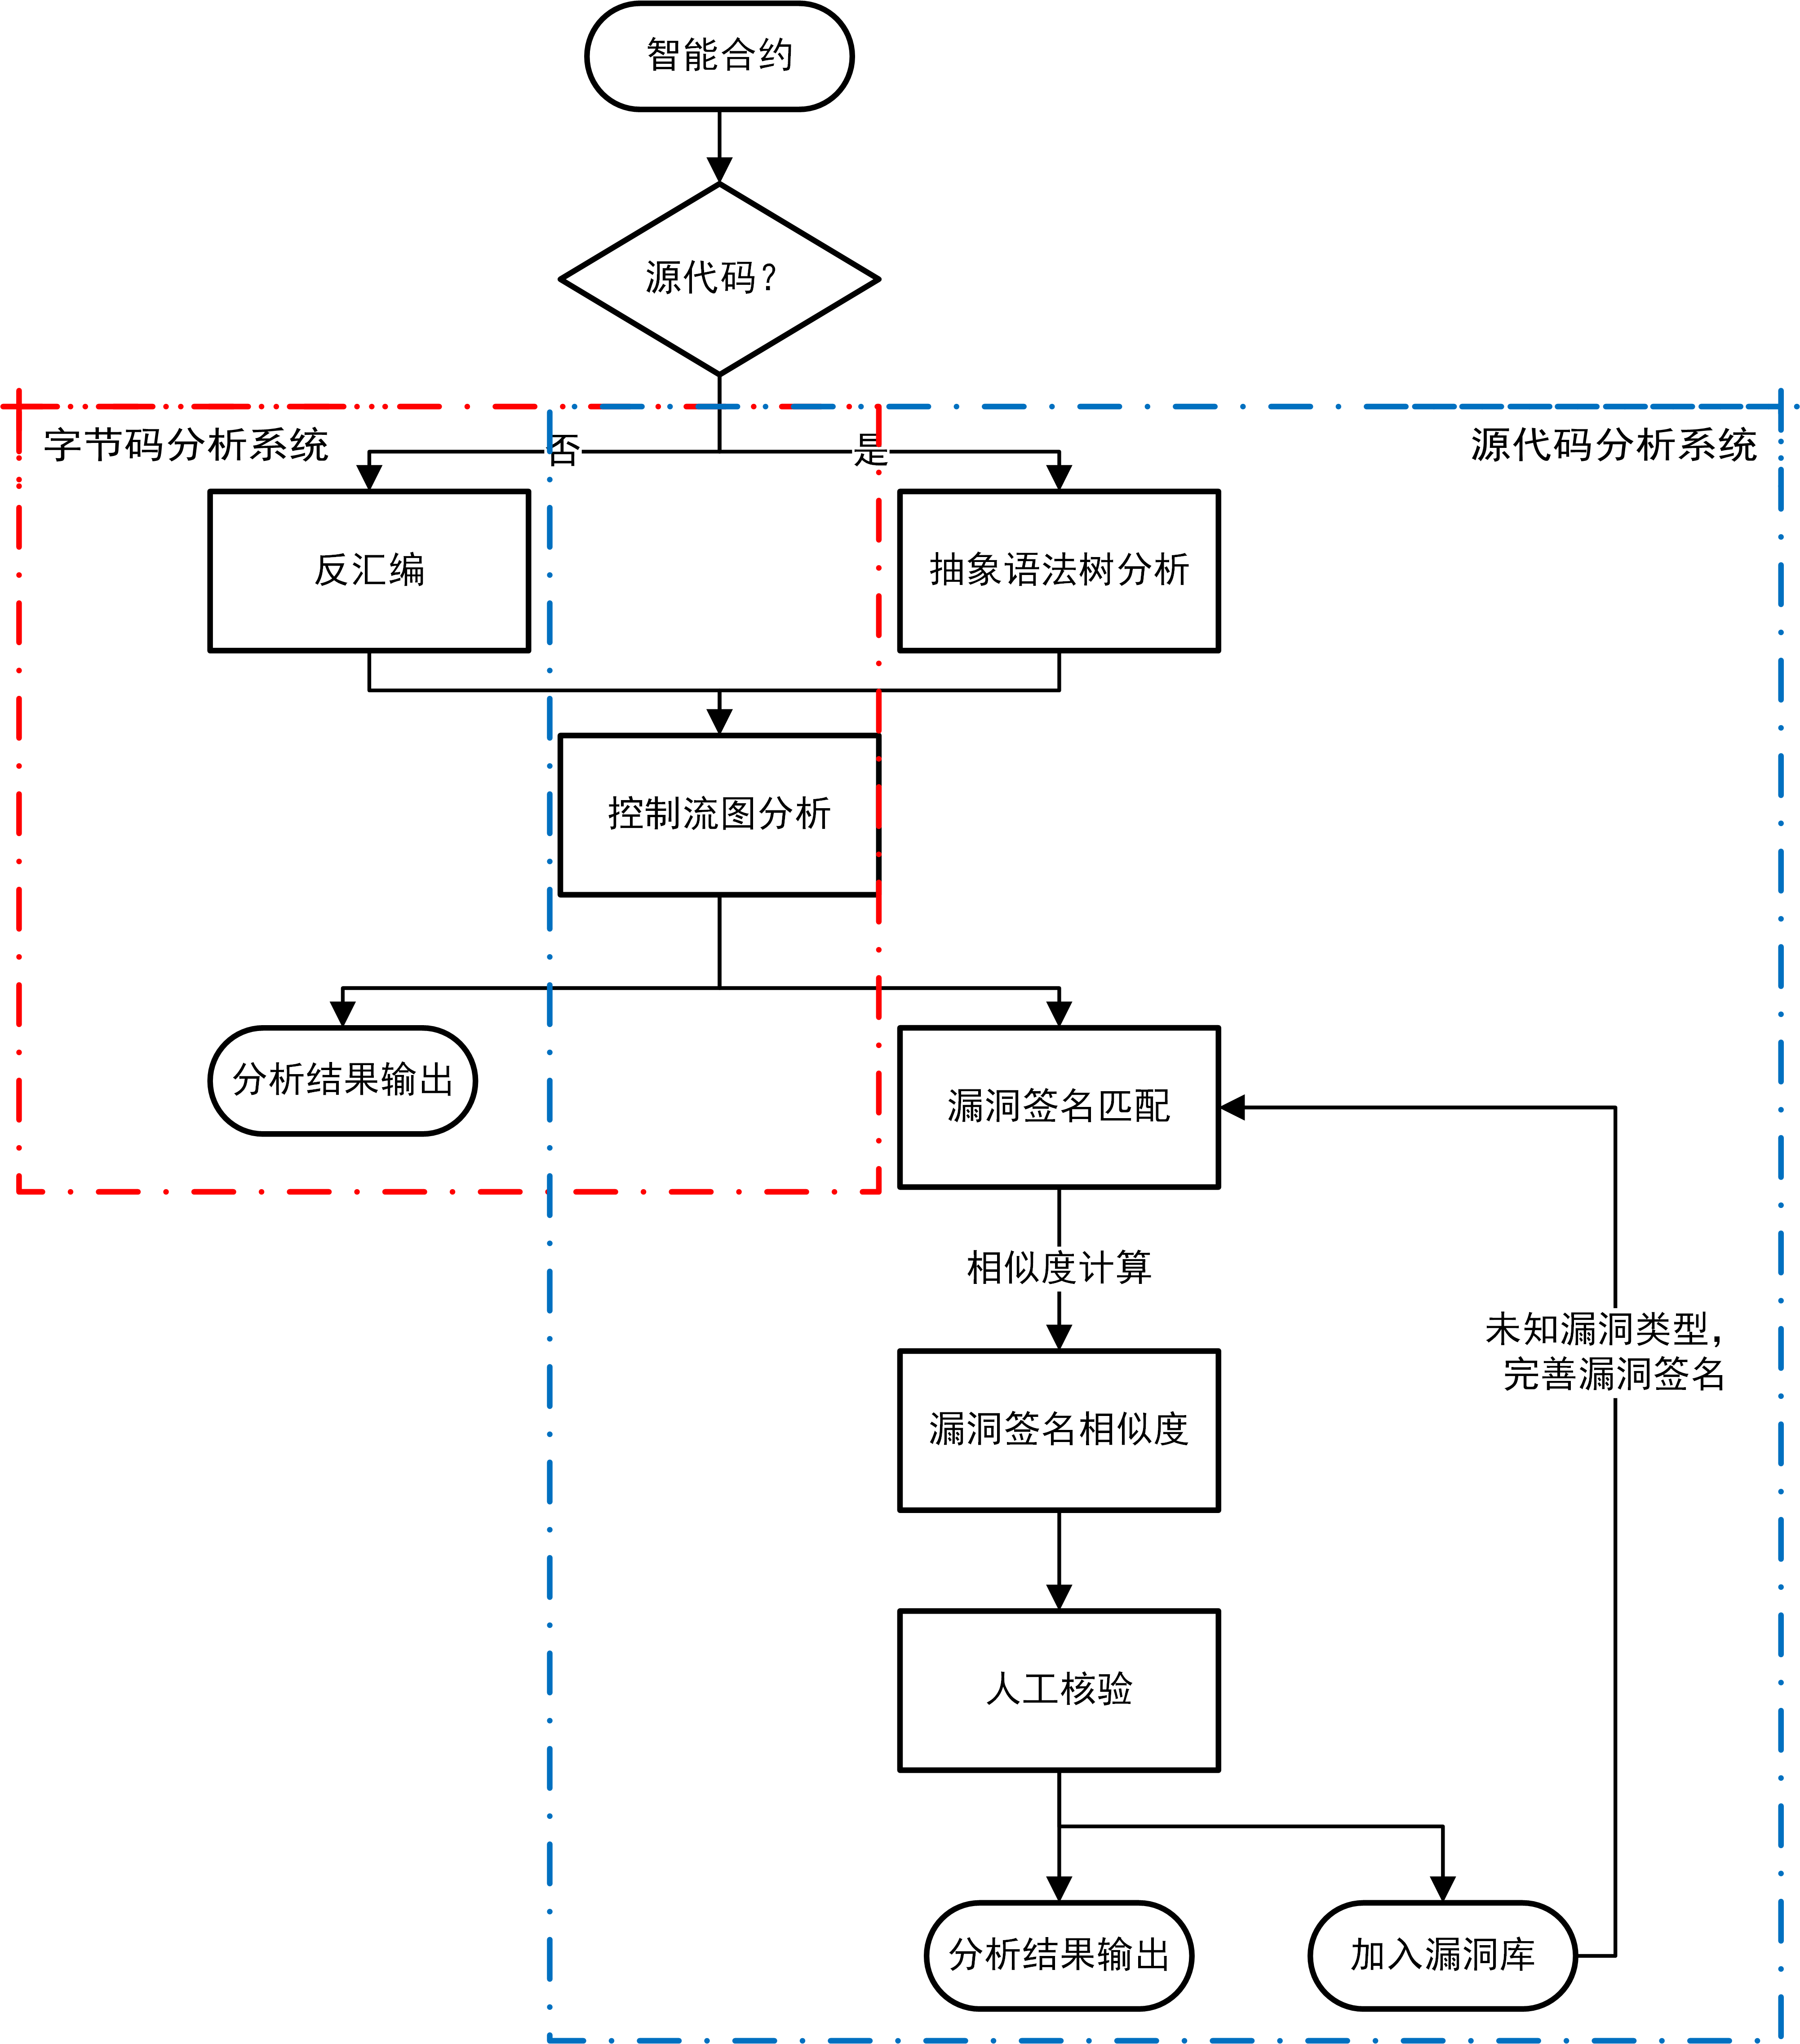
\includegraphics[width=0.8\textwidth]{figures/system_diagram.png}
  \caption{漏洞检测系统结构设计图}
  \label{fig:system_diagram}
\vspace{-5mm}
\end{figure}

\section{基于规则的漏洞检测技术}\label{sec:detection_rules}

对于我们需要研究的主要漏洞,我们需要从现有的漏洞示例和现有工具的检测策略中不断学习,加上我们的领域专家对以太坊平台及智能合约的认识,总结归纳出漏洞的检测规则,以便于之后使用克隆分析技术在漏洞检测规则的基础上寻找漏洞代码。对于现有的几个开源工具,我们可以通过阅读源代码的方式去研究他们的实现原理,分析他们的制定的漏洞规则的优缺点,不断完善我们的漏洞检测规则。在本节,我们将针对不同的漏洞进行分析,并得到适合用作克隆分析技术的漏洞检测规则。

\subsection{可重入漏洞检测规则}
对于影响力巨大的可重入漏洞,\textsc{Slither}在实现中使用的检测器是以式\ref{rule:slither: reentrance}为规则进行检测的。
\begin{mdframed}[
	linewidth = 1pt,
	innertopmargin = -5pt,
	innerbottommargin = 3pt,
	outerlinewidth = 1pt
	]
	\begin{equation} \label{rule:slither: reentrance}
	\small
	r(var_{global}) \wedge (operation_{sendeth}) \wedge r(var_{global}) \Rightarrow \text{\emph{Reentrancy}}
	\end{equation}
\end{mdframed}
\textsc{Slither}在检测可重入漏洞时,会首先检查控制流图中的全局变量读操作,即$r(var_{global})$,这一步是因为全局变量在以太坊中有着重要的作用。由于以太坊的底层运行是基于操作栈实现的,全局变量在以太坊通常是以\codeff{public}类型修饰,作用域包括整个合约。因此,对于全局变量的操作容易带来安全隐患,而对全局变量的读取操作则是对全局变量修改的第一步。\textsc{Slither}重视对全局变量的敏感操作,因此会检查对全局变量的读取和写入操作。更进一步,为了保证检测规则的准确性,\textsc{Slither}优先检查涉及转账操作$operation_{sendeth}$的全局变量修改,因为在转账操作周围的全局变量读写操作通常会带来收到漏洞攻击危险。\textsc{Slither}在控制流图上进行分析,控制流图的每个块内部都是中间语言形式的代码语句,这种中间语言在源代码的基础上做了一定程度的抽象,有利于\textsc{Slither}无视无关代码进行准确的漏洞检测。

\textsc{Oyente}的检测规则如式\ref{rule:oyente: reentrance}所示。
\begin{mdframed}[
	linewidth = 1pt,
	innertopmargin = -5pt,
	innerbottommargin = 3pt,
	outerlinewidth = 1pt
	]
    \small
	\begin{equation} \label{rule:oyente: reentrance}
    \begin{split}
       r(var_{global}) \wedge (gas_{trans} > 2300) \wedge \big (type(var_{amount}) == type(var_{global})\big )  \\
       \Rightarrow \text{\emph{Reentrancy}}
    \end{split}
	\end{equation}
\end{mdframed}
\textsc{Oyente}的检测规则和\textsc{Slither}有很大的不同,因为\textsc{Oyente}是对智能合约的字节码进行检测的工具。对字节码反编译过后的中间语言建立控制流图,并进行分析。因为字节码的操作码和操作所消耗的\codeff{gas}是一一对应的,如表\ref{tab:opcode_gas}所示,因此,对字节码进行分析可以分析函数的\codeff{gas}消耗,这是以源代码为输入的分析方式所做不到的。同时,\textsc{Oyente}检查了外部调用操作消耗的\codeff{gas}是否超过2300,这是因为可重入漏洞的一个最大的特点就是针对重复调用并不断消耗\codeff{gas}。如果发现了外部调用大于2300这个阈值,则很有可能发生了重入。最后,\textsc{Oyente}检查了交易的金额变量是否为全局变量。这是因为全局变量经常涉及敏感操作,而控制转账金额的变量决定了受害者受到的损失的大小。\textsc{Oyente}的规则要求控制转账金额的变量必须不为全局变量。

\textsc{Securify}的检测规则如式\ref{rule:securify: reentrance}所示。\textsc{Securify}的检测规则相比\textsc{Slither}和\textsc{Oyente}要简单很多。\textsc{Securify}是基于\emph{Datalog}语言做的符号执行分析,它会在检测漏洞之前将智能合约字节码转换成\emph{Datalog}语言。\textsc{Securify}在检查可重入漏洞时,会检查语句块内部有没有外部调用和对全局变量的操作,避免发生敏感操作。其次,如果检测器发现对全局变量的操作没有放在外部调用之前,检测器会报告这是一个可重入漏洞。\textsc{Securify}的检测逻辑简单易懂,它抓住全局变量和外部调用的先后关系进行检测,\emph{Datalog}语言也对产出准确的检测结果有一定的帮助。但是,相比其他两个工具,\textsc{Securify}的检测模式还是过于简单和粗暴,这可能会带来很多的误报。
\begin{mdframed}[
	linewidth = 1pt,
	innertopmargin = -5pt,
	innerbottommargin = 3pt,
	outerlinewidth = 1pt
	]
    \small
	\begin{equation} \label{rule:securify: reentrance}
    external\_call \wedge w(var_{global}) \wedge (\text{ write must follow the call})  \Rightarrow \text{\emph{Reentrancy}}
	\end{equation}
\end{mdframed}
通过对其他三个工具的观察和我们对智能合约漏洞的理解,我们认为,一个完备的可重入漏洞规则,应该是如式\ref{rule:athena: reentrance}所示。在我们的检测规则中,我们没有采用\textsc{Oyente}的检测规则中对操作消耗\codeff{gas}检查,因为我们的检测工作是面向源代码而不是字节码, 在源代码上做\codeff{gas}消耗分析会产生很多困难;我们也没有采用\textsc{Securify}中对于外部调用和全局变量操作的前后关系进行检测的规则,因为我们觉得这个规则容易带来误报。我们吸取了\textsc{Slither}的检测规则中对交易操作与全局变量写入操作的检查,并加入了没有\codeff{gas}限制的危险调用的检查。这是因为早期的\codeff{call}、\codeff{delegatecall}等低级调用如果不加限制,很容易带来重入隐患。如果出现没有\codeff{gas}限制的危险调用,我们就可以认为这能够带来一定的漏洞隐患;同时如果出现在转账操作之后有相关的全局变量写入操作,我们也认为会带来漏洞隐患。
\begin{mdframed}[
	linewidth = 1pt,
	innertopmargin = -10pt,
	innerbottommargin = 3pt,
	outerlinewidth = 1pt
	]
    \small
	\begin{equation} \label{rule:athena: reentrance}
    \begin{split}
       \big ((dangerous\_call) \wedge (no\_gas\_limit)\big ) \vee \big ((operation_{sendeth}) \wedge w(var_{global})\big ) \\
       \Rightarrow \text{\emph{Reentrancy}}
    \end{split}
	\end{equation}
\end{mdframed}

\subsection{意外异常漏洞检测规则}

意外漏洞多发生于在\codeff{for}或者\codeff{while}循环中进行交易操作的情况,账户持有者向其他人循环发送金额,如果在循环中的某一次转账操作发生异常导致转账异常,则后面的数次转账操作都将被取消。这个漏洞容易被黑客用于DoS攻击,如果黑衣故意在转账过程中加入异常代码,使得整个交易次数取消,就达到了拒绝服务攻击的目的。

对于意外异常漏洞,支持的工具有\textsc{Slither}、\textsc{Smartcheck}和我们的系统\textsc{Athena},而\textsc{Oyente}和\textsc{Securify}因为是在字节码的基础上做进一步分析,很难抓取到这个漏洞的特点,因此这两个工具不具备检查这个漏洞的功能。\textsc{Slither}对于这个漏洞的检测规则如式\ref{rule:slither: revert}所示。
\begin{mdframed}[
	linewidth = 1pt,
	innertopmargin = -5pt,
	innerbottommargin = 3pt,
	outerlinewidth = 1pt
	]
    \small
	\begin{equation} \label{rule:slither: revert}
    (has\_loop) \wedge (calls\_inside) \Rightarrow \text{\emph{Unexpected Revert}}
	\end{equation}
\end{mdframed}

在式中,\textsc{Slither}首先检查控制流图中的循环结构,如\codeff{for}或者\codeff{while}循环,然后检查在循环结构的内部是否包含外部调用语句。在检查外部调用的时候,\textsc{Slither}检查高级外部调用(即用户定义的函数的调用)、低级调用以及转账函数\codeff{send}和\codeff{transfer}。如果有其中任何一种调用出现在循环结构内,\textsc{Slither}则判定这段代码含有意外异常漏洞。

\textsc{Smartcheck}检测意外异常漏洞的规则如式\ref{rule:smartcheck: revert}所示。
\begin{mdframed}[
	linewidth = 1pt,
	innertopmargin = -5pt,
	innerbottommargin = 3pt,
	outerlinewidth = 1pt
	]
    \small
	\begin{equation} \label{rule:smartcheck: revert}
    \begin{split}
       \big ((if) \wedge (revert\_inside)\big ) \vee \big ((for) \wedge (calls\_inside)\big ) \\
       \Rightarrow \text{\emph{Unexpected Revert}}
    \end{split}
	\end{equation}
\end{mdframed}
\textsc{Smartcheck}在处理意外异常错误的时候会检查两种情况,一种是\codeff{if}语句和函数体内部有没有\codeff{revert},如果同时成立则有了抛出异常的可能性,引发意外异常漏洞;一种是在\codeff{for}循环语句的内部是否包含外部调用,如果外部调用失败则有可能会造成意外异常错误。\textsc{Smartcheck}和其他工具不同的地方是把\codeff{revert}也当作漏洞检测规则的一部分,在我们看来\codeff{revert}多用于需要抛出异常的函数体内,属于正常的业务逻辑,不能被归纳为漏洞的一部分。同时,\textsc{Smartcheck}对一切的外部调用一视同仁,只要出现在\codeff{for}循环内部则判断为有漏洞,这种判断规则在我们看来,有些过于简单和武断。

在观察过其他两个工具对于意外异常漏洞的检测规则后,我们制定我们系统的检测规则如式\ref{rule:athena: revert}所示。
\begin{mdframed}[
	linewidth = 1pt,
	innertopmargin = -5pt,
	innerbottommargin = 3pt,
	outerlinewidth = 1pt
	]
    \small
	\begin{equation} \label{rule:athena: revert}
    (for \vee while) \wedge \big ((require \wedge send) \vee transfer \big )  \Rightarrow \text{\emph{Unexpected Revert}}
	\end{equation}
\end{mdframed}
在我们的规则中,我们首先检查函数体是否包含\codeff{for}或者\codeff{while}循环语句,再检查函数体内部有没有\codeff{require}语句和\codeff{send}语句,如果没有的话再检查函数体内部是否包含\codeff{transfer}语句。我们制定这样的检测规则是因为\emph{Solidity}的部分内建语句自带了抛出异常功能。例如,\codeff{transfer}语句有抛出异常的功能,而\codeff{send}语句没有。所以如果使用\codeff{send}语句,当调用执行失败,\codeff{send}会返回\codeff{false},但不会抛出异常。如果\codeff{send}语句外部有\codeff{require}函数对交易的执行结果进行检验,\codeff{send}语句就具备了抛出异常的功能,也就有了触发意外异常漏洞的风险。

\subsection{低级调用漏洞检测规则}
低级调用漏洞主要是由低级漏洞自身的安全检查不完备造成的。多数低级调用,如\codeff{call}、\codeff{delegatecall}都是\emph{Solidity}语言诞生初期的产物。这些低级调用实现了最基本的功能,但缺少了一些安全检查,导致使用这些低级调用的行为变成引发漏洞的行为。\emph{Solidity}不推荐开发者使用这些低级调用函数,如果实在有使用的需要,要求开发者在低级调用的外部加上\codeff{require}、\codeff{assert}等检查函数。如果低级调用执行失败,这些检查函数会收到低级调用的返回值\codeff{false},并抛出异常终止整个合约的运行。

\textsc{Slither}对于这种低级调用漏洞的检测规则如式\ref{rule:slither: llc}所示。
\begin{mdframed}[
	linewidth = 1pt,
	innertopmargin = -5pt,
	innerbottommargin = 3pt,
	outerlinewidth = 1pt
	]
    \small
	\begin{equation} \label{rule:slither: llc}
    ( call) \vee (delegatecall) \vee (send) \Rightarrow \text{\emph{Unchecked Low Level Call}}
	\end{equation}
\end{mdframed}
\textsc{Slither}对于这个漏洞的检查规则非常简单粗暴,它检查函数控制流图上所有的低级调用操作,一旦出现低级调用,就判断函数出现低级调用漏洞。毋庸置疑,这会给\textsc{Slither}在这个漏洞的检测任务上带来很高的误报率。

\textsc{Smartcheck}对与这种低级调用漏洞的检测规则如式\ref{rule:smartcheck: llc}所示。
\begin{mdframed}[
	linewidth = 1pt,
	innertopmargin = -5pt,
	innerbottommargin = 3pt,
	outerlinewidth = 1pt
	]
    \small
	\begin{equation} \label{rule:smartcheck: llc}
    (if) \wedge \big ((call) \vee (delegatecall) \vee (send) \big ) \Rightarrow \text{\emph{Unchecked Low Level Call}}
	\end{equation}
\end{mdframed}
\textsc{Smartcheck}对于这个漏洞会首先检查\codeff{if}语句的使用,如果出现了这个语句,再检查语句内部是否包含\codeff{call}、\codeff{delegatecall}或者\codeff{send}这三个低级调用,如果有的低级调用没有被包含在\codeff{if}语句内部则判断代码包含低级调用漏洞。\textsc{Smartchecl}认为只有\codeff{if}语句才能算作检查,而忽略了\codeff{require}、\codeff{assert}这两种检查函数,这会忽略掉很多真正的漏洞。

在观察其他两个工具对低级调用漏洞的检测规则之后,我们制定了我们的系统的检测规则如式\ref{rule:athena: llc}所示。
\begin{mdframed}[
	linewidth = 1pt,
	innertopmargin = -5pt,
	innerbottommargin = 3pt,
	outerlinewidth = 1pt
	]
    \small
	\begin{equation} \label{rule:athena: llc}
    \begin{split}
       \big ((call) \vee (delegatecall) \vee (send)\big ) \wedge without \big ((require) \vee (assert) \vee (if)\big )  \\
        \Rightarrow \text{\emph{Unchecked Low Level Call}}
    \end{split}
	\end{equation}
\end{mdframed}
我们的规则覆盖了主要的低级调用如\codeff{call}、\codeff{delegatecall}和\codeff{send},同时也附加了对几种主要的检查函数\codeff{require}、\codeff{assert}和\codeff{if}的检查。我们认为\textsc{Slither}的规则会产生很多误报,因为它的规则过于武断,没有对检查函数的检查环节;我们也认为\textsc{Smartcheck}的规则也是不完备的,因为它只检查\codeff{if}这一个检查函数,而没有覆盖其他的两个检查函数,这也会对检查结果产生影响。在分析以上两个工具的规则的优缺点之后,我们设计了自己的检查规则。

\subsection{自毁漏洞检测规则}
自毁漏洞是也是由于函数的正常功能在不正当使用条件下使用产生的。\codeff{selfdestruct}函数实在\emph{Solidity}语言设计之初就加入的函数,它停止当前的任何功能,清空\codeff{gas},并把当前合约剩余的余额全部转移至其他合约。这个内建函数有一个参数,即转移余额的地址。这个函数本属于智能合约正常交易周期的一部分,负责在合约完成其生命周期之后清理剩余的合约资源,避免合约当中的资源浪费。但是,如果这个函数没有受到严格的调用限制,比如在特定的时间、特定的运行次数或者特定的访问者调用,甚至转账的地址是不受到合约的持有者控制的,这个函数就会引发自毁漏洞。攻击者触发函数,停止合约的当前功能,并向攻击者的账户转移所有财产。

\textsc{Slither}对于这个漏洞的检查规则如式\ref{rule:slither: suicidal}所示。
\begin{mdframed}[
	linewidth = 1pt,
	innertopmargin = -5pt,
	innerbottommargin = 3pt,
	outerlinewidth = 1pt
	]
    \small
	\begin{equation} \label{rule:slither: suicidal}
    (selfdestruct) \wedge (func_{public}) \wedge (access\_available) \Rightarrow \text{\emph{Suicidal}}
	\end{equation}
\end{mdframed}
\textsc{Slither}在检查这个漏洞时候,首先检查这个函数受否包含\codeff{selfdestruct}自毁函数,其次检查包括这个自毁函数的外部函数修饰符是否是\codeff{public},最后检查这个自毁函数是否能被轻易到达。\textsc{Slither}的检测规则目前已经比较完备,但还有一点不足,\textsc{Slither}这样的检查方式会把正常的业务逻辑也判为漏洞代码。因为正常的业务代码函数体积较大,在函数的最后有自毁函数,这个函数符合\textsc{Slither}的检测规则,但是它对自毁函数的使用是正确的。

为了改正\textsc{Slither}的一点缺陷,我们提出我们系统的检查规则如式\ref{rule:athena: suicidal}所示。
\begin{mdframed}[
	linewidth = 1pt,
	innertopmargin = -10pt,
	innerbottommargin = 3pt,
	outerlinewidth = 1pt
	]
    \small
	\begin{equation} \label{rule:athena: suicidal}
    \begin{split}
       (selfdestruct) \wedge (func_{public}) \wedge (access\_available) \wedge (func_{selfdestruct}) \\
       \Rightarrow \text{\emph{Suicidal}}
    \end{split}
	\end{equation}
\end{mdframed}
我们的检测规则在\textsc{Slither}的基础上加入了新的要求,我们要求只有当检测的函数为自毁函数体,即只包含自毁功能的函数时,我们才判断这个函数为漏洞函数。这个规则修正了\textsc{Slither}把很多正常的业务逻辑误判为漏洞的缺陷,降低了系统的误报率。

\section{使用安全盾降低系统误报数}\label{sec:ss}

安全盾(Security Shield)指开发者在开发过程中使用特定的技术保护代码不受漏洞侵害的技术。在确定针对不同漏洞的检测规则之后,我们可以借助克隆检测技术,在程序的控制流图上寻找符合漏洞检测规则的代码。如果出现了符合规则的代码,则将这段代码报告为漏洞代码。这样做确实能获取大量的疑似漏洞代码,但却不能保证这些疑似漏洞代码真实存在漏洞。很明显,在\ref{sec:detection_rules}节中,我们归纳了针对不同漏洞的众多规则,可是这些检测规则缺乏对上下文语境的考虑,也没法保证检测规则是完美无缺的,因此在实际操作中,尽管我们的规则已经针对现有规则做出了相当的改进,但是仍会有很高的误报率。如图\ref{fig:ss_example}中代码所示。
\begin{figure}
\begin{minipage}[htb]{1.0\linewidth}
    \begin{lstlisting}
    contract buyOne {
        constructor{
            owner = msg.sender
        }
        ...
        function buy(address target, uint amount) public {
            require(msg.sender == owner);
            target.call.value(amount);
            ...
        }
    }
    \end{lstlisting}
    %\caption{test}
\end{minipage}
\vspace{-5mm}
\caption{安全盾实例,开发者借助图中第7行的身份验证,有效防止可重入攻击}
\label{fig:ss_example}
\end{figure}
代码中的\codeff{owner}地址在构造器\codeff{constructor}中被赋值,而构造器只有在合约软件初始化时才能被调用,故\codeff{owner}变量一定是合约创建者的地址。在函数中\codeff{buy}中,第7行检查了合约访问者\codeff{msg.sender}与\codeff{owner}地址是否相等。这不起眼的一行,有效地阻止了可重入攻击。

在我们阅读Solidity源代码,分析程序执行情况的过程中,我们发现有大量优秀的开发者,在开发智能合约软件的时候遵守了软件的开发规范,使得智能合约软件具备了防范漏洞攻击的能力。这些防范技术各有差异,虽然可以把它们大致分为几类,但它们个体之间的实现差异较大,这不利于克隆技术的实现,会带来很高的误报率。这是由于克隆分析技术的特性决定的。事实上,在其他软件平台,漏洞代码和安全代码之间的差异可能会变得很小,过于相似的代码导致克隆分析技术无法直接对这些代码做出准确判断。因此,在我们的检测系统中,我们将加入安全盾技术,通过这项技术减少现有克隆分析技术可能带来的高误报数,提高系统检测漏洞的准确率。在接下来的几小节中,我们将针对我们使用的安全盾技术进行阐述。其中,对于可重入漏洞,我们总结了SS1-SS5,对于意外异常漏洞,我们总结了SS6-SS7,对于低级调用漏洞,我们总结了SS8,对于自毁漏洞,我们总结了SS9。

\subsection{SS1:在函数体中加入身份检查}

SS1通过简单的方法就实现了限制函数访问的功能。很多开发者在编写函数的功能的时候,会在实际的功能代码前面加入相关的身份检查,检查合约的访问者是否是合约的持有者或者是否合法。实现身份检查有多种形式,我们举例一种形式如图\ref{fig:ss1_example}所示。
\begin{figure}
\begin{minipage}[htbp]{1.0\linewidth}
    \begin{lstlisting}
    function finalize() public initialized {
        require(finalizedBlock == 0);
        require(finalizedTime == 0);
        require(getBlockTimestamp() >= startTime);
        require(msg.sender == controller || getBlockTimestamp() > endTime);

        uint256 tokenCap = aix.totalSupply().mul(100).div(51);
        aix.generateTokens(devHolder, tokenCap.mul(20).div(100));
        aix.generateTokens(communityHolder, tokenCap.mul(29).div(100));
        ...
    }
    \end{lstlisting}
    %\caption{test}
\end{minipage}
\vspace{-5mm}
\caption{SS1:在函数体中加入身份检查}
\label{fig:ss1_example}
\end{figure}
在图\ref{fig:ss1_example}中,代码的第3-6行实现了四种检查功能,其中在第6行通过检查\codeff{msg.sender == controller}来限制对该函数访问。\codeff{controller}是一个全局变量,在合约的构造函数中被赋值,这意味着他只能由创建者进行赋值,无法被其他人更改。在这里这个函数检查了访问这身份是否是\codeff{controller},这也就意味着这段代码只能被合约的持有者执行。在很多情况下,执行转账操作、自毁操作时,合约的创建者希望函数功能由创建者本人或者创建者信任的访问者执行,他们通过添加身份检查实现了这个功能。
\subsection{SS2:限制转账的目标地址}

开发者也可以通过限制转账的目标地址来进行可重入攻击的防御。目标的转账地址通常都是由一个全局变量进行维护或者通过函数的传参进行更新,如果不注意转账地址的限制,攻击者就可以采用多种方式修改转账的目标地址,改为自己的账户地址进而通过\codeff{fallback}函数进行重入攻击。在Solidity开发过程中,对与转账地址的管理,一定要慎之又慎。通常,开发者可以通过限制转账地址,即采用硬编码的方式制定转账的目标地址,或者限制转账地址的修改,即只允许部分访问者有权利更改转账的目标地址这两种方式去防御可重入攻击。如图\ref{fig:ss2_example}中代码所示。
\begin{figure}
\begin{minipage}[htbp]{1.0\linewidth}
    \begin{lstlisting}
    contract Etherama{
        constructor() public {
            require(dataContractAddress != address(0x0));
            _data = EtheramaData(0x00a2409f41fdf485afd23599219c60a77524bba2);
            ...
            creator = msg.sender;
        }
        function changeData(address newAddress) public {
            require(msg.sender == creator);
            _data = EthermaData(newAddress);
        }
        function migrateToNewNewControllerContract() public {
            uint256 remainingTokenAmount = getRemainingTokenAmount();
            ...
            _data.transfer(remainingTokenAmount);
            ...
        }
    }
\end{lstlisting}
%\caption{test}
\end{minipage}
\vspace{-5mm}
\caption{SS2:限制转账的目标地址}
\label{fig:ss2_example}
\end{figure}
在图中,函数在第11行向\codeff{\_data}进行转账操作 ,而这个全局变量在函数构造器\codeff{constructor}里面进行初始化,初始化时,这个初始化函数使用了一个20位的16进制的地址,即合约账户在以太坊平台上的绝对地址进行了赋值,故这个转账的目标地址在一开始是被限制死的。随后,虽然函数中准备了更改目标转账地址的函数\codeff{changeData}可以进行\codeff{\_data}数据的修改,但是在这个修改函数的一开始就使用了\codeff{require}函数进行了身份验证,限制了修改函数的操作必须由\codeff{creator}执行,而和\codeff{\_data}一样,这个\codeff{creator}的地址也是在构造器中进行的初始化,外来的访问者是无法随意突破这道屏障的。总的来说,这个合约的开发者虽然提供了转账操作、修改地址等功能,但是对涉及转账目标地址的操作,每一步都设置了防范措施,在这些防范措施的保护下,合约的转账地址很难被攻击者肆意修改。

\subsection{SS3;使用函数修饰器限制访问}\label{sec:ss3}
SS3的原理和SS1很像,相比SS1在函数体中直接进行身份检查,SS3把这个实现放到里函数修饰器里。函数修饰器是Solidity语言的特点之一。Solidity语言提供\codeff{internal}、\codeff{private}、\codeff{public}等内建修饰符限制对函数的访问,除此之外,Solidity还允许开发者使用\codeff{modifier}模块自行设计函数修饰器。自定义函数修饰器中通常都有下划线\codeff{\_;},表明修饰目标函数的原函数体。将自定义修饰符添加至函数原型上,执行时通常将优先执行修饰器内部的功能,然后再执行原函数体。因为自定义修饰符的这个特性,开发者们将身份验证的模块写入函数修饰器内部,保证在执行时,先通过修饰器内部的身份检查函数检查访问者的身份,再执行函数的具体功能。如图\ref{fig:ss3_example}中的代码所示。
\begin{figure}
\begin{minipage}[htbp]{1.0\linewidth}
    \begin{lstlisting}
    contract ShortOrder is SafeMath {
        modifier onlyAdmin() {
            require(msg.sender == admin);
            _;
        }
        ...
        function claims(address[2] tokenUser, address usr, uint amount) external onlyAdmin {
            bytes32 orderHash = keccak256(tokenUser[0],tokenUser[1]);
            ...
            usr.transfer(safeAdd(orderRecord[orderHash],amount));
            Token(tokenUser[0]).transfer(admin,orderRecord[orderHash]);
            orderRecord[orderHash].balance = uint(0);
            ...
        }
    }
\end{lstlisting}
%\caption{test}
\end{minipage}
\vspace{-5mm}
\caption{SS3:使用函数修饰器限制访问}
\label{fig:ss3_example}
\end{figure}
图中的函数第2-4行实现了修饰器\codeff{onlyAdmin},在修饰器的开始使用了\codeff{require}语句检查访问者的身份,限制函数仅允许合约的管理员访问。这是个简单的函数修饰器实例。随后这个修饰器被用于\codeff{claimDonations}上。这个函数在第10行向由函数参数传入的\codeff{usr}账户进行转账,本来直接使用函数传参用于转账操作是一种容易引发漏洞的高发行为,但是通过使用\codeff{onlyAdmin}修饰符,每次在执行这个函数之前都要检查函数的访问者是否为合约的管理者,有效地阻止了函数被攻击者恶意利用。

\subsection{SS4:使用程序的执行锁防止重入}
使用程序锁防止重入是一种比较巧妙的技术,通常开发者会设置一个互斥变量用作执行锁,在每次执行关键操作之前先检查执行锁的值,并修改执行锁的现有值,再进行正常的业务操作。这种防范方式会在攻击者第二次试图进入函数时挡住攻击者,因为执行锁的值已经在第一次运行时改变了,在第二次运行时无法通过执行锁值的检查,进而达到防止程序被重入的效果。在图\ref{fig:ss4_example}中,函数10行进行执行锁的检查,在第11行更改了锁的值,在更改执行锁的值之后再在第12行进行转账操作。如果有攻击者试图使用重入进行函数攻击,那么在第二次重入时,攻击者将无法通过程序执行锁的检查,也无法进行可重入攻击。因此,这个安全盾技术通过简单的代码即实现了对可重入攻击的防范。
\begin{figure}
\begin{minipage}[htbp]{1.0\linewidth}
    \begin{lstlisting}
    contract MicroDAO{
        bool public executed = false;
        ...
        function execute() internal {
            ...
            executed=false;		
        }
        function executeSpendingRequests(address _addr, uint amount) public payable {
            MicroDAO m =MicroDAO(allowances[_addr]);
            if(!executed) {
                m.execute();
                _addr.transfer(amount);
                ...
            }
        }
    }
    \end{lstlisting}
%\caption{test}
\end{minipage}
\vspace{-5mm}
\caption{SS4:使用程序的执行锁防止重入}
\label{fig:ss4_example}
\end{figure}

\subsection{SS5:提前更新状态变量}
这种防御手段主要是在转账之前更新状态变量(即转账金额),这样在进行重入时,状态变量已经发生了改变,攻击者无法通过状态变量的检查,进而达到防御可重入攻击的目的。如图\ref{fig:ss5_example}所示,图中代码在第6行进行转账操作,但在转账操作之前,第5行进行余额的检查,而余额时在第3行进行赋值的,被赋值为\codeff{balanceOf}数组中访问者的余额,在赋值完成之后,随即把数组中访问者的余额赋值为0,并马上进行转账操作。在经过这样的预先处理之后,攻击者在第二次重入时,数组中访问者的余额已经被赋值为0了,故攻击者无法通过第5行的余额检查。这个函数通过对余额的检查以及在转账之前进行状态变量的更新成功达到了防范可重入漏洞攻击的目的。
\begin{figure}
\begin{minipage}[htbp]{1.0\linewidth}
    \begin{lstlisting}
    function safeWithdrawlal() public companyCanBeFinished{
        if (!fundingGoalReached){
            uint amount = balanceOf[msg.sender];
            balanceOf[msg.sender] = 0;
            if (amount > 0){
                msg.sender.send(amount);
                FundTransfer(msg.sender, amount, false)
            }
            ...
        }
    }
    \end{lstlisting}
%\caption{test}
\end{minipage}
\vspace{-5mm}
\caption{SS5:提前更新状态变量}
\label{fig:ss5_example}
\end{figure}

\subsection{SS6:不在循环语句中使用检查函数}\label{sec:ss6}

根据我们观察,在循环语句中对\codeff{send}使用\codeff{require}会容易导致意外异常漏洞。这是因为在Solidity语言中,\codeff{send}语句转账失败时会返回\codeff{false}而不抛出异常,而\codeff{transfer}在语句转账之后会检查返回结果,如果返回结果为\codeff{false}则自动抛出异常。如果我们使用\codeff{send}配合\codeff{require}做检验,那么会导致在转账失败时,合约失去服务能力,进而发生拒绝服务的行为。因此,Solidity开发者们为了阻止由\codeff{send}语句引发的漏洞攻击,不会使用\codeff{require}检查\codeff{send}转账的结果。

\subsection{SS7:在循环语句中向单个地址进行转账}\label{sec:ss7}

在智能合约软件代码中,有些业务逻辑使用循环语句向单个账户地址发送一定金额的以太币。这种情况下,如果某次转账失败,导致整个循环转账的业务逻辑中断,我们也不会判断这个代码是包含漏洞的代码。因为我们在考虑漏洞代码的特征时,不仅要考虑代码本身的攻防逻辑,也要考虑在实际情况中的应用场景。不符合实际应用场景的攻击逻辑,即便可以轻松达到攻击代码的目的,我们也不认为这是一个漏洞代码。在此处这个向单个用户发送以太币的情况下,如果在循环中有单词转账失败导致整个业务的暂停,业务的暂停也不会影响到别的账户,不符合拒绝服务攻击的应用场景,因此我们把这归纳为安全盾技术的一种,我们认为不对他人造成任何侵害的代码不应该属于漏洞代码。

\textcolor[rgb]{1.00,0.00,0.00}{Add code example}

\subsection{SS8:使用多种检查方式检查低级调用}\label{sec:ss8}

Solidity语言诞生之初带来的诸多低级调用函数被开发者们诟病久矣。这些低级调用接近底层,有诸多使用限制,对Solidity语言不够熟练的开发者很容易在使用低级调用时埋下安全隐患。Solidity在后面的迭代过程中,推出了很多高级的外部调用来替代低级调用的功能,这些高级调用对低级调用中极少使用但容易埋下漏洞隐患的部分做了封装,让用户能更安全地使用这门语言进行开发。如果开发者一定有使用低级调用的必要,也需要配合\codeff{assert}、\codeff{require}、\codeff{if}等检查语句一并使用,保证低级调用的失败得到妥善处理,也保证智能合约软件的业务逻辑能正常进行。

\subsection{SS9:在使用自毁函数时增加严格的身份检查}\label{sec:ss9}

自毁函数\codeff{selfdestruct}具有很强的攻击性,在使用不当的情况下很容易造成漏洞攻击。我们观察大量代码之后,认为防范这种漏洞引发的攻击最好的方法便是增加严格的身份检查功能。通过函数修饰符或者直接在函数体内部实现身份检查都能防止自毁函数被任意的访问者调用,增加函数的安全性。

\textcolor[rgb]{1.00,0.00,0.00}{Add code example}

\section{漏洞检测算法设计}

\begin{algorithm}[htbp]
	\small
	% 	\SetAlgoLined
	\SetKwInOut{Input}{输入}
	\SetKwInOut{Output}{输出}
    \Input{
        \\
        $S$, 针对某漏洞的函数签名\;\\
        $C$, 被检测的目标代码\;\\
        $\eta$, 代码相似度上界\;\\
        $\gamma$, 代码相似度下界\;\\
        $itv$, 检测窗口变化率\;\\
        }
	\Output{$V$, 漏洞函数集\;}
    $w \leftarrow LineofCode(C)$ \\
    $c \leftarrow CodeofWindow(w,C)$ \\
    $F \leftarrow FunctionList(c)$ \\
    $V \leftarrow \emptyset$ \\
    \For {each function $f \in F$} {
        \uIf { $Similarity(S,c) \le \gamma$ }{
            $w \leftarrow w \times itv$ \\
            $c \leftarrow CodeofWindow(w, C) $ \\
        }
        \ElseIf { $Similarity(S,c) \ge \eta$ }{
            $w \leftarrow w \times \frac{1}{itv}$ \\
            $c \leftarrow CodeofWindow(w, C) $ \\
        }
        \ElseIf{$Similarity(S,c) \in (\gamma,\eta)$}{
            $V \leftarrow V \vee f$ \\
        }
    }
    \For { each vulnerable candidates $v \in V$} {
        \For { each rule $r \in SecurityShields$} {
            $b \leftarrow Match(r, v)$ \\
            \uIf {$b == True$} {
                $V \leftarrow V - v$ \\
            }
        }
    }
	\caption{基于代码克隆分析的漏洞检测算法}\label{algo:matching}
\end{algorithm}


在获取了漏洞的漏洞签名和用于减低误报率的安全盾技术之后,我们提出我们的漏洞检测算法如算法\ref{algo:matching}所示。我们设计的算法总共有五个输入,其中$S$为针对某函数的漏洞签名,我们使用漏洞签名来匹配疑似漏洞的代码;$C$为被检测的代码,即待检测代码;$\eta$和$\gamma$分别为代码相似度的上界和下界,这两个值是人为预先设定,并根据系统的表现不断调整的,它们决定了寻找克隆代码窗口的调整大小;$itv$为每次调整窗口的变化率,变化率越大则窗口大小的改变越激进。输出有一个,即漏洞检测算法找到的漏洞函数集合。

在算法的前面四行,我们将$w$的初始值设置为整段代码的大小,$c$设置为在这段代码上的窗口扫描到的代码,$F$为窗口扫描到的代码中的所包含的函数列表,$V$为初始为空集。在函数的第一个循环5-15行,我们遍历了函数列表中的每个函数,并对每一个函数和漏洞签名使用了相似度算法——最长公共子串(Longest Common Subsequence)算法计算相似度,如果相似度过高,说明可能窗口值过大,我们需要按照一定的变化率调整窗口的大小并重新扫描;如果相似度过低,则说明窗口值过小,我们需要放大窗口的大小并重新扫描;如果相似度在相似度上界和下界之间,则说明窗口值刚好,有很大可能匹配到了漏洞代码,我们把匹配成功的函数加入漏洞函数集。

在算法的第二个循环16-22行,我们对漏洞集$V$中的每个漏洞候选进行遍历,用我们在上一节\ref{sec:ss}中介绍的安全盾去一一匹配,如果和安全盾匹配的相似度高,则说明这个代码对相应的漏洞做出了一定程度的防范,不在我们的考虑范围之列,并在第20行将代码从我们的漏洞集中去除。

这个算法最大时间开销来自于算法的第5-15行,首先我们使用循环语句遍历每个函数,并使用LCS算法进行相似度计算,时间复杂度为$\mathcal{O}(n^{3})$。而在算法的第二个循环即17-23行,我们虽然使用了两层遍历,但是在计算是否匹配时我们使用基于规则的匹配技术,综合时间复杂度为$\mathcal{O}(n^{2})$。我们设计的算法并不是最快的,但是得益于智能合约体积软件体积较小,尚没有举行的智能合约软件出现,即便我们使用了如此高时间复杂度的算法,我们在Solidiity软件上检测漏洞的时间开销也不会太高。
